\section{Design consequences and comparison of preparations}\label{sec:design}
\subsection{Capacity, initial filling and retained renewal}
Table~\ref{tab:examples} compares the certified preparations under the same administration, the same amount $32.48$ and the same horizon $120$. The original small-reserve estimate uses the top anchor and a narrower target box: chemistry factors in $[.9999,1.0001]$, division within $10^{-5}$ of $.1$, and each baseline death within $10^{-5}$ of its nominal value. Its weighted error is at most $.001w$, giving target risk below $.00535$. The wide-box results spend some of that probability margin to allow one-percent relative error in all these target rates. They also change capacity and selectivity, so the reduction of the renewal requirement from $12$ to $1$ is \emph{not} a comparison at otherwise identical parameters; it is a statement about what a different preparation buys.

\begin{table}[tb]
\centering\small
\caption{Certified preparations. All rows have $\nu\in[0,.005]$, clearance $k_e\in[.99,1.01]$, four $AA$ founders, horizon $120$ and the same delivered course~\eqref{eq:course}. Healthy renewal may exceed the displayed minimum. The displayed probabilities are separate marginal upper bounds, not exact risks.}\label{tab:examples}
\setlength{\tabcolsep}{4pt}
\begin{tabular}{@{}lrrrrlrl@{}}
\toprule
Preparation & $K$ & $h_{\min}$ & $H_0\ge$ & $\reff\ge$ & $\sigma$ & Healthy loss & Source\\
\midrule
Original benchmark    & 20  & 10  & 20  & 12 & $[1,2]$ & $5.0\times10^{-4}$ & \\
Same capacity         & 20  & 10  & 20  & 9  & $[1,2]$ & $8.5\times10^{-3}$ & \\
Larger reserve        & 400 & 200 & 278 & 1  & $[2,3]$ & $7.0\times10^{-6}$ & Thm.~\ref{thm:main}\\
Lower filling         & 400 & 200 & 240 & 1  & $[2,3]$ & $2.9\times10^{-6}$ & Cor.~\ref{cor:filling}\\
Minimal filling       & 400 & 200 & 209 & 1  & $[2,3]$ & $9.8\times10^{-3}$ & Cor.~\ref{cor:filling}\\
Smaller reserve       & 232 & 116 & 161 & 1  & $[2,3]$ & $9.8\times10^{-3}$ & Cor.~\ref{cor:smaller}\\
\bottomrule
\end{tabular}
\medskip
\begin{tabular}{@{}lll@{}}
\toprule
Preparation & Target uncertainty & Target survival\\
\midrule
Original benchmark; same capacity & Narrow mixed relative/absolute box & $0.00535$\\
All wide-box rows & Independent one-percent relative box & $0.00856$\\
\bottomrule
\end{tabular}
\end{table}

The three wide-box rows separate two resources that are easy to conflate. The \emph{lower filling} row shows that the $278$-unit anchor of Theorem~\ref{thm:main} buys margin rather than feasibility: the certificate degrades gracefully, and it is only near $209$, nine units above the failure threshold, that the mission tolerance is actually reached. The \emph{smaller reserve} row shows the complementary trade: shrinking capacity by $42\%$ at fixed proportions consumes essentially the same margin. Increasing $K$ and increasing $H_0/K$ enter different terms of the guarantee, the first through the product in~\eqref{eq:anchorbound} and the second through the initial scale term in~\eqref{eq:initial}. Figure~\ref{fig:scaling} displays the two dependences side by side.

For $K=400$, the return level $278$ is close to the equilibrium count under the worst comparison source, $400(1-.305)=278$. Anchoring there rather than at the ceiling is what makes the certificate usable: an excursion is not required to return to an atypical hard ceiling that a treated reserve rarely visits. Theorem~\ref{thm:anchor} remains valid above this level even when the initial reserve is not full, and Corollary~\ref{cor:initial} quantifies depleted or random preparation rather than silently resetting the reserve.

If intervention inhibits renewal, only the retained lower rate enters the certificate. In particular a nominal $r=2$ with retained fraction $\chi_{\min}=1/2$ meets $\reff\ge1$. This is a quantitative sufficient condition on renewal retained \emph{during} exposure; it does not assert that any particular intervention has that property, and renewal measured without treatment is not the relevant quantity.

\begin{figure}[tb]
 \centering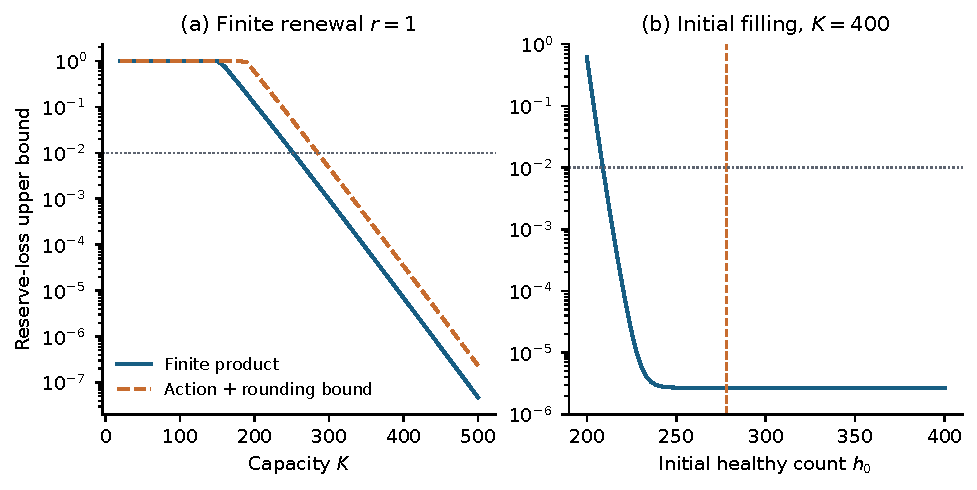
\includegraphics[width=.94\linewidth]{figures/capacity_and_filling.pdf}
 \caption{Two distinct reserve resources. (a) Finite-product and action bounds for $m=.305$, $\reff=1$, threshold $\lceil K/2\rceil$ and initial count at least $\lfloor.695K\rfloor$, through $T=120$. (b) The initial-state scale-function bound at $K=400$, threshold $200$, anchor $278$. Increasing capacity and increasing initial filling change different terms of the guarantee. The horizontal dotted line is risk $.01$; the sharp knee in (b) near $h_0\approx210$ is the content of Corollary~\ref{cor:filling}. Curves are evaluations of proved bounds, clipped at one.}\label{fig:scaling}
\end{figure}

\subsection{Founder burden and finite mission limits}
The weight~\eqref{eq:w} gives $z_0\cdot w/w_{\min}\le10.7n$ for any $n$ initial target cells, regardless of their types. A four-unit ramp followed by a contraction interval of length $\ell$ therefore has the sufficient target bound
\begin{equation}\label{eq:burden}
 \Prob(|Z_{4+\ell}|>0)\le10.7\,n\exp(4g-\gamma\ell),\qquad
 \ell\ge\gamma^{-1}\left[\log\frac{10.7n}{\delta}+4g\right],
\end{equation}
with zero sufficing when the displayed requirement is negative. For the fixed course of Theorem~\ref{thm:main} the coarser rational bound is $107n/50000$, which certifies $n\le4$ at $\delta=.01$. The dependence on burden is only logarithmic, but the proof does not cover arbitrary burden at fixed amount and deadline, because a longer course is a different course: administration lasts $4+\ell$ and requires amount $.29(4+\ell)$, concentration-exposure allowance at least $.29(4+\ell)/.99$, and a horizon including the declared washout. All three limits must be enlarged explicitly, and the enlarged horizon then feeds back into the reserve requirement. Substituting that horizon into~\eqref{eq:sizing} links capacity to founder burden through the logarithmic contraction duration. Alternatively the top-anchor product gives the sufficient renewal requirement
\begin{equation}\label{eq:renewalsizing}
 \reff\ge Km\left(\frac{KmT}{\alpha\,d!}\right)^{1/d},\qquad
 d=K-h_{\min}\ge1,\quad H_0=K.
\end{equation}
By Proposition~\ref{prop:highrenewal} this rule has the right order: the bound it inverts is asymptotically exact as $\reff\to\infty$, so no argument of this type can improve its $\alpha^{-1/d}$ or $(d!)^{-1/d}$ dependence by more than a factor tending to one. It remains a sufficient resource law rather than a necessary one, and capacity, initial filling, renewal, selectivity and target burden should be kept as separate coordinates in any design comparison.

\begin{figure}[tb]
 \centering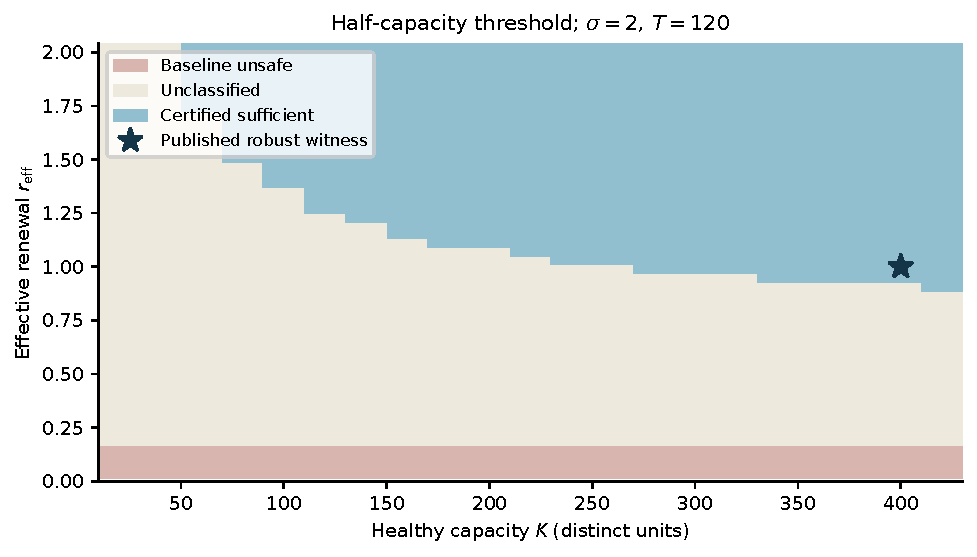
\includegraphics[width=.94\linewidth]{figures/capacity_design_map.pdf}
 \caption{A sufficient design map, not an optimal frontier. At each displayed $(K,\reff)$ a return level is selected and its finite-product inequality is checked rationally at $m=.305$, $h_{\min}=K/2$, $T=120$; the sufficient region assumes initial count at least that selected level. Combined with the wide-box target certificate, blue points satisfy both $.01$ tolerances. The red band is already unsafe from baseline mortality $.15$ at $\sigma=2$ even when initially full; its classification uses the expectation bound of Section~\ref{sec:limits}. The remaining region is unclassified, not proved infeasible. The star is Theorem~\ref{thm:main}.}\label{fig:map}
\end{figure}

\section{What the guarantee does and does not establish}\label{sec:limits}
\subsection{Baseline failure is different from treatment-induced failure}
The original small-reserve excluded example has $K=H_0=20$, $h_{\min}=10$, $\sigma\le2$ and $r\le.001$. For any nonnegative intervention, healthy per-unit mortality is at least $.15$ while births are at most $rh$. Therefore
\[
 \mathcal G H\le-(.15-.001)H=-.149H,\qquad
 \Prob(H_{120}\ge10)\le\frac{\E H_{120}}{10}\le2e^{-17.88}<10^{-7},
\]
so path failure exceeds $1-10^{-7}$ under every policy. This is a genuine all-policy obstruction, but it reflects \emph{baseline} reserve collapse: the reserve in that region dies without any treatment at all. It is therefore no evidence of a sharp treatment-induced selectivity boundary. More generally, when mortality is at least $m_0>\reff$ and births are at most $\reff h$, survival above threshold is at most $(H_0/h_{\min})e^{-(m_0-\reff)T}$, and this elementary test is what labels the baseline-unsafe band of Figure~\ref{fig:map}.

\subsection{The safe-baseline converse is open}\label{sec:converse}
The interesting question left open is the converse in the complementary region: if the untreated reserve is safe, is there a source for which \emph{no} admitted policy achieves both tolerances? We do not resolve it, and we record why the natural approach fails, since the obstruction is concrete.

A standard route seeks a generator subsolution certifying an upper bound on joint success. With $W=1-q^z$ for a product supersolution $q$, the target generator satisfies $\mathcal G_CW\ge-(67v/73+k)W$, where $v$ and $k$ are the delivered rate levels; one then looks for $e^{-\eta(T-t)}f(h)W$ with $0\le f\le1$ and $\mathcal G_Hf+(\eta-67v/73-k)f\ge0$ on all safe states. Because the constraint is affine in the rate levels, exact vertex testing on the admissible rectangle covers all trajectories. The attempt fails for a structural reason rather than a numerical one. Under the normalization $f(K)=1$, births vanish at the ceiling, so the $K$-state row forces
\[
 \eta\ \ge\ \frac{67\cdot\tfrac3{10}}{73}+\frac1{10}=0.37534\ldots,
\]
which is incompatible with the discount range in which the remaining rows admit a solution. Raising the failure penalty cannot repair this row, since it does not appear there. Eighteen exact linear programs over three renewal values and six discounts returned no separating objective beyond the zero function. This is an algebraic obstruction to that ansatz, not a theorem that a therapeutic window does or does not exist; closing the question needs a subsolution retaining more source, control or budget information. The sufficient mission theorem and the capacity law do not depend on it, and we therefore make no global frontier claim and no constant-versus-varying optimality claim.

\subsection{Immediate regeneration is a substantive assumption}
At a hard ceiling with $h_{\min}=K$ the first healthy death is already failure. Since $\lambda_K=0$, renewal cannot act before that event, and per-unit mortality at least $m_0$ gives failure probability exactly $1-e^{-Km_0T}$ for constant mortality, regardless of $\reff$. With a positive buffer the top-anchor bound instead tends to zero as $\reff$ grows, at the exact rate given by Proposition~\ref{prop:highrenewal}. The discontinuity at $d=0$ belongs to the specified jump model.

Delayed replenishment can impose a risk floor even with a buffer. Suppose no replacement can complete during an initial latency $\tau\le T$, there is no preloaded maturation pipeline, $H_0=K$, and mortality is at least $m_0$ per unit during that interval. Pure-death comparison gives
\begin{equation}\label{eq:latency}
 \Prob(\tau_H\le T)
 \ge\Prob\{\operatorname{Bin}(K,e^{-m_0\tau})<h_{\min}\},
\end{equation}
independently of subsequent renewal, by coupling the actual deaths above independent rate-$m_0$ deaths before the first replenishment is available; recovery after a crossing cannot undo the path event. At $K=20$, $h_{\min}=10$ and $e^{-m_0\tau}=1/2$ this floor exceeds $0.41$. A loaded pipeline changes the hypothesis and may remove the floor. Myelosuppression models already distinguish proliferating, maturation-transit and circulating compartments \citep{friberg}; immediate logistic replenishment should not be equated with such recovery dynamics, and~\eqref{eq:latency} is the precise price of that idealization.

\subsection{Dimensionless meaning and empirical requirements}
Table~\ref{tab:meaning} records the main scales in units of nominal target division $b=.1$. A time-unit conversion leaves these ratios unchanged, so ``renewal one'' is a statement about a ratio, not evidence of a physiological timescale: the new renewal ratio is ten rather than the original $120$, and it remains an uncalibrated assumption.
\begin{table}[tb]
\centering\small
\caption{Scales and quantities that would require empirical identification. No clinical units are inferred.}\label{tab:meaning}
\begin{tabularx}{\linewidth}{@{}l l >{\raggedright\arraybackslash}X@{}}
\toprule
Quantity & Nominal value or ratio & Meaning / required information\\
\midrule
Renewal / division & $\reff/b=10$ at the new lower bound & Retained renewal during exposure, not untreated renewal alone\\
Clearance / division & $k_e/b\in[9.9,10.1]$ & Actual clearance and effect-site response\\
Healthy mortality / division & $m/b\le3.05$ & Shared injury and healthy baseline loss\\
Target mortality / division & $d_i/b\in\{.1,3\}$ nominally & State-specific baseline event rates\\
Reserve threshold & $h_{\min}/K=.5$ & Functional threshold and independently specified count units\\
Initial reserve & $H_0/K\ge.695$, or $\ge.5225$ by Cor.~\ref{cor:filling} & Actual filling or preparation distribution\\
Target inheritance & Equation~\eqref{eq:pairs} & Joint daughter allocation, not only mean trajectories\\
Uncertainty & Relative errors $\le1\%$ on the rates of Rem.~\ref{rem:box} & A mathematical box requiring external justification\\
Maturation & No delay in the main source & Transit time and initial pipeline if present\\
\bottomrule
\end{tabularx}
\end{table}

The most informative experiments are those that test a comparison assumption rather than sweep schedules: whether renewal remains above the needed floor under exposure, whether the delivered response actually enters the contraction band, and whether replenishment has a latency incompatible with the mission. Any one of these can invalidate the model faster, and more informatively, than a large dosing grid. Joint daughter-state observations matter for the same reason: matching mean inheritance is not sufficient, because a replacement kernel with the same $L$ can change extinction probabilities.

The intervention acts on a literal inherited-state population, while the reserve law is a birth--death mechanism with its own probabilistic origin. The capacity results are therefore not \emph{caused} by epigenetic inheritance, and should not be described that way. The distinct contributions are the finite-reserve certificate, the source-specific inherited-population contraction, and their composition under one delivered input. Together these identify properties that a hypothetical intervention and preparation would need. They do not establish the safety of any available drug, prescribe a regimen, or predict a patient's outcome.
